\subsection{Conjuntos de Cantor}

\begin{frame}
\vspace{5pt}
\frametitle{Família Quadrática: Conjuntos de Cantor}
\begin{columns}
\column{\dimexpr\paperwidth-15pt}

Se $\mu > 4$, então existem pontos em $[0, 1]$ cujas órbitas não estão contidas em $[0, 1]$. Portanto, seja
$$\Lambda_n = \lbrace x \in [0, 1] : h^n(x) \in [0, 1] \rbrace$$ 
para cada $n \geq 1$. Definindo
$$\Lambda =  \bigcap_{n = 1}^\infty \Lambda_n,$$
podemos restringir o estudo da dinâmica de $h$ em $\Lambda$.

\end{columns}
\end{frame}

%--------------------

\begin{frame}
\frametitle{Família Quadrática: Conjuntos de Cantor}
\begin{columns}
\column{\dimexpr\paperwidth-15pt}

\begin{proposition}
Se $\mu > 4$, então
\begin{enumerate}
\item $\Lambda_n$ é a união de $2^n$ intervalos fechados disjuntos.
\item $h^n: [a, b] \to [0, 1]$ é bijetora, onde $[a, b]$ é um dos intervalos que formam $\Lambda_n$.
\end{enumerate}
\end{proposition}

\begin{figure}[!htb]
\centering
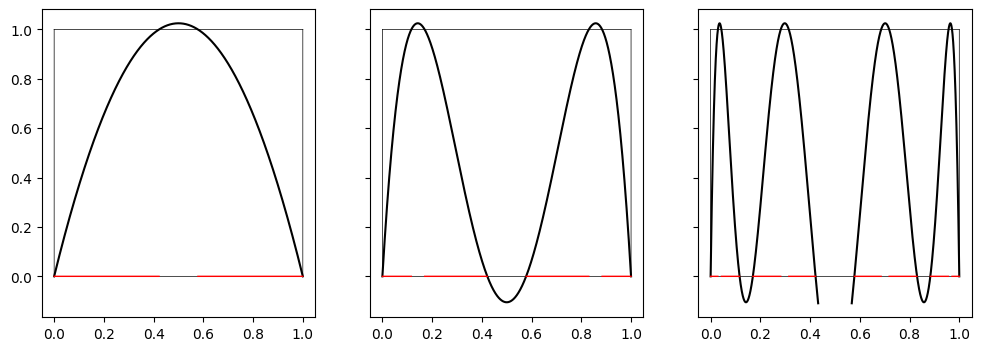
\includegraphics[scale=0.4]{images/h_4,1.png}
\caption{Gráficos de $h$, $h^2$ e $h^3$ para $\mu = 4.1$.}
\label{h_3,839}
\end{figure}

\end{columns}
\end{frame}

%--------------------

\begin{frame}
\vspace{5pt}
\frametitle{Família Quadrática: \subsecname}
\begin{columns}
\column{\dimexpr\paperwidth-15pt}

Para facilitar as demonstrações, consideramos $\mu > 2 + \sqrt{5}$.

\begin{lemma}
Se $\mu > 2 + \sqrt{5}$, então existe $\nu > 1$ tal que
\begin{enumerate}
\item  $|D h(\Lambda_1)| > \nu$,
\item $b - a < \frac{1}{\nu^n}$, onde $[a, b]$ é um dos intervalos que formam $\Lambda_n$.
\end{enumerate}
\end{lemma}

\vspace{10pt}

\begin{theorem}
Se $\mu > 2 + \sqrt{5}$, então $\Lambda$ é um conjunto de Cantor.
\end{theorem}

\begin{block}{Observação}
Esse teorema é válido para $4 < \mu \leq 2 + \sqrt{5}$, porém a demonstração é mais complicada.
\end{block}

\end{columns}
\end{frame}
